\chapter{平面几何}


\section{运动与曲线}
\subsection{圆沿着曲线滚动}
\subsubsection{沿直线滚动}
\paragraph*{摆线}圆沿着一条直线滚动,其边上一点形成的曲线叫摆线。
假设初始时圆心坐标为$(0,r)$,初始的圆上的点为$(0,0)$。从几何角度推导如下图:

\begin{center}
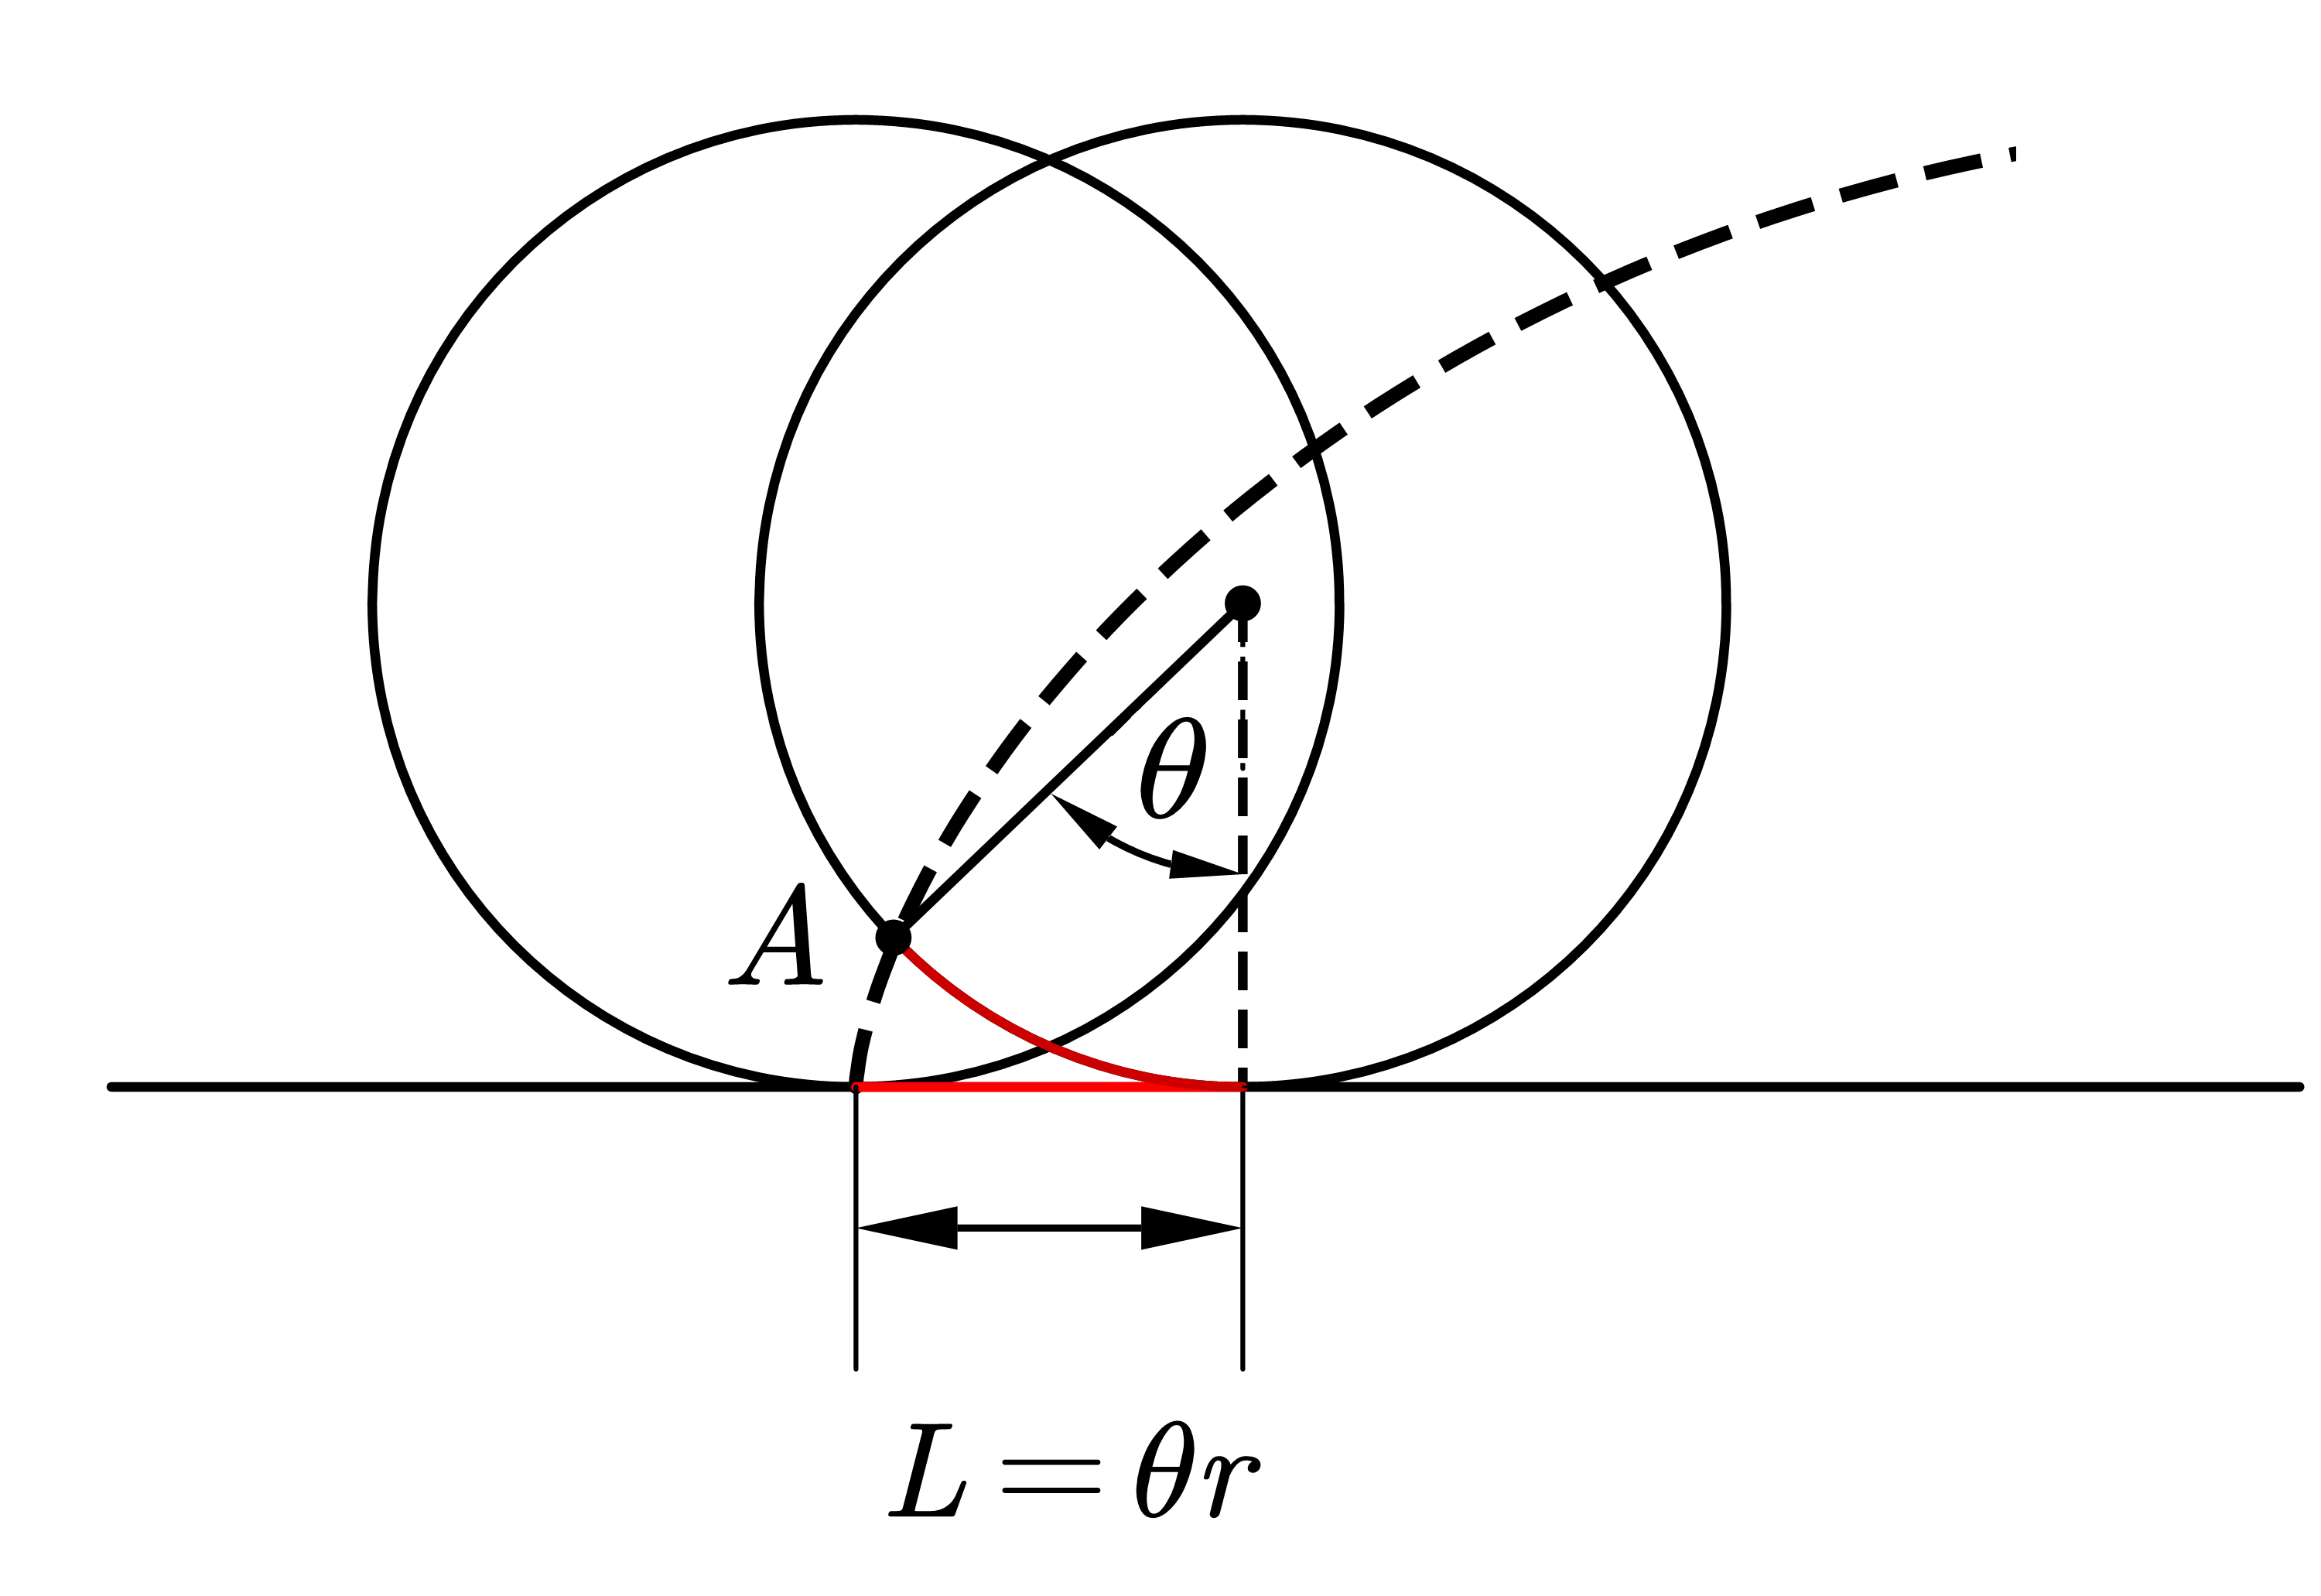
\includegraphics[width=8cm]{figure/摆线.png}
\end{center}

图中两段红线的长度应该是相等的。求$A$点的坐标时可以先把圆心平移到圆点,此时坐标为
\begin{empheq}{align*}
x&=r\cos\sbra{-\frac{\pi}{2}-\theta}\\
y&=r\sin\sbra{-\frac{\pi}{2}-\theta}
\end{empheq}
再平移回去,$x$坐标增加$L=r\theta$,$y$坐标增加$r$。即有:
\begin{empheq}{align*}
	x&=r\sbra{\theta-\sin\theta}\\
	y&=r\sbra{1-\cos\theta}
\end{empheq}

从另一个角度来看,假如沿直线滚动了长度$L$,那么我们需要在圆上找一点,使得其弧长恰好也是$L$。

\subsubsection{沿圆滚动}
如下图所示,小圆沿着大圆滚动:

\begin{center}
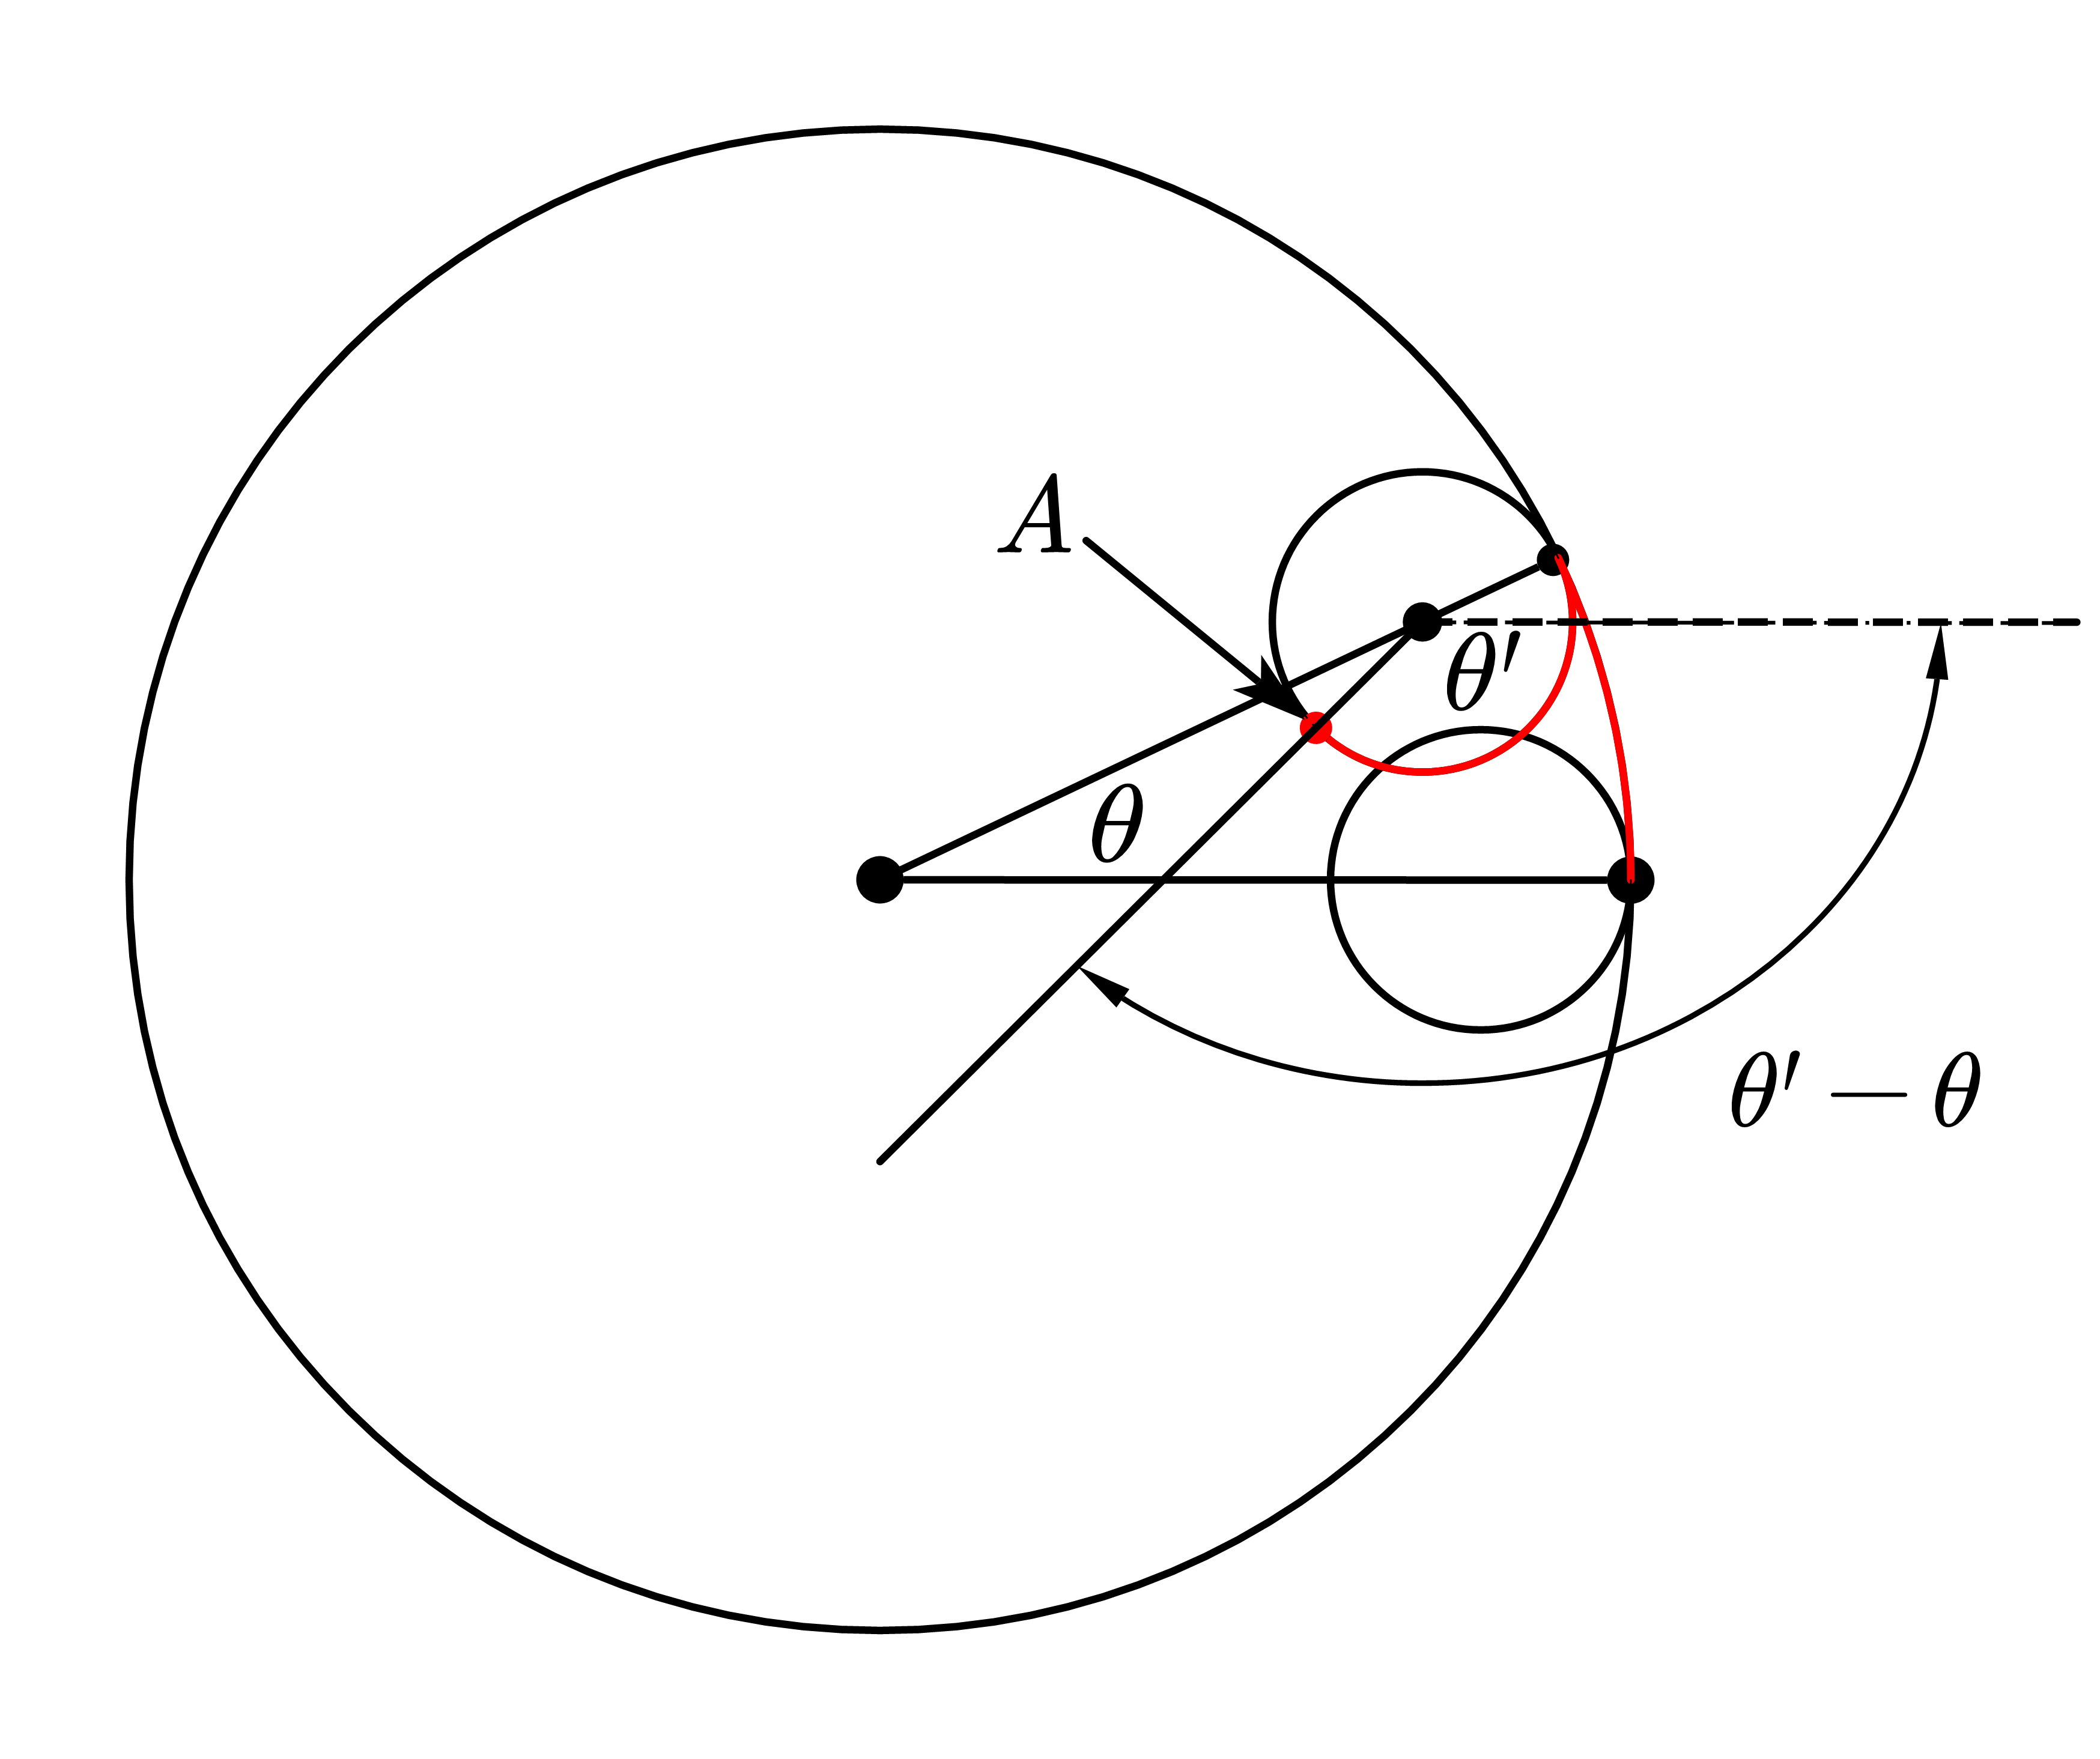
\includegraphics[width=8cm]{摆线(圆上).png}
\end{center}

计算时可以没用找弧长为$L$的方法。

